%%%%%%%%%%%%%%%%%%%%%%%%%%%%%%%%%%%%%%%
% Wenneker Resume/CV
% LaTeX Template
% Version 1.1 (19/6/2016)
%
% This template has been downloaded from:
% http://www.LaTeXTemplates.com
%
% Original author:
% Frits Wenneker (http://www.howtotex.com) with extensive modifications by 
% Vel (vel@LaTeXTemplates.com)
%
% License:
% CC BY-NC-SA 3.0 (http://creativecommons.org/licenses/by-nc-sa/3.0/
%
%%%%%%%%%%%%%%%%%%%%%%%%%%%%%%%%%%%%%%

%----------------------------------------------------------------------------------------
%	PACKAGES AND OTHER DOCUMENT CONFIGURATIONS
%----------------------------------------------------------------------------------------

\documentclass[a4paper,12pt]{memoir} % Font and paper size

%%%%%%%%%%%%%%%%%%%%%%%%%%%%%%%%%%%%%%%%%
% Wenneker Resume/CV
% Structure Specification File
% Version 1.1 (19/6/2016)
%
% This file has been downloaded from:
% http://www.LaTeXTemplates.com
%
% Original author:
% Frits Wenneker (http://www.howtotex.com) with extensive modifications by 
% Vel (vel@latextemplates.com)
%
% License:
% CC BY-NC-SA 3.0 (http://creativecommons.org/licenses/by-nc-sa/3.0/)
%
%%%%%%%%%%%%%%%%%%%%%%%%%%%%%%%%%%%%%%%%%

%----------------------------------------------------------------------------------------
%	PACKAGES AND OTHER DOCUMENT CONFIGURATIONS
%----------------------------------------------------------------------------------------

\usepackage{XCharter} % Use the Bitstream Charter font
\usepackage[utf8]{inputenc} % Required for inputting international characters
\usepackage[T1]{fontenc} % Output font encoding for international characters

\usepackage[top=1cm,left=1cm,right=1cm,bottom=1cm]{geometry} % Modify margins

\usepackage{graphicx} % Required for figures

\usepackage{flowfram} % Required for the multi-column layout

\usepackage{url} % URLs

\usepackage[usenames,dvipsnames]{xcolor} % Required for custom colours

\usepackage{tikz} % Required for the horizontal rule

\usepackage{enumitem} % Required for modifying lists
\setlist{noitemsep,nolistsep} % Remove spacing within and around lists

\setlength{\columnsep}{\baselineskip} % Set the spacing between columns

% Define the left frame (sidebar)
\newflowframe{0.2\textwidth}{\textheight}{0pt}{0pt}[left]
\newlength{\LeftMainSep}
\setlength{\LeftMainSep}{0.2\textwidth}
\addtolength{\LeftMainSep}{1\columnsep}
 
% Small static frame for the vertical line
\newstaticframe{1.5pt}{\textheight}{\LeftMainSep}{0pt}
 
% Content of the static frame with the vertical line
\begin{staticcontents}{1}
\hfill
\tikz{\draw[loosely dotted,color=RoyalBlue,line width=1.5pt,yshift=0](0,0) -- (0,\textheight);}
\hfill\mbox{}
\end{staticcontents}
 
% Define the right frame (main body)
\addtolength{\LeftMainSep}{1.5pt}
\addtolength{\LeftMainSep}{1\columnsep}
\newflowframe{0.7\textwidth}{\textheight}{\LeftMainSep}{0pt}[main01]

\pagestyle{empty} % Disable all page numbering

\setlength{\parindent}{0pt} % Stop paragraph indentation

%----------------------------------------------------------------------------------------
%	NEW COMMANDS
%----------------------------------------------------------------------------------------

\newcommand{\userinformation}[1]{\renewcommand{\userinformation}{#1}} % Define a new command for the CV user's information that goes into the left column

\newcommand{\cvheading}[1]{{\Huge\bfseries\color{RoyalBlue} #1} \par\vspace{.6\baselineskip}} % New command for the CV heading
\newcommand{\cvsubheading}[1]{{\Large\bfseries #1} \bigbreak} % New command for the CV subheading

\newcommand{\Sep}{\vspace{1em}} % New command for the spacing between headings
\newcommand{\SmallSep}{\vspace{0.5em}} % New command for the spacing within headings

\newcommand{\aboutme}[2]{ % New command for the about me section
\textbf{\color{RoyalBlue} #1}~~#2\par\Sep
}
	
\newcommand{\CVSection}[1]{ % New command for the headings within sections
{\Large\textbf{#1}}\par
\SmallSep % Used for spacing
}

\newcommand{\CVItem}[2]{ % New command for the item descriptions
\textbf{\color{RoyalBlue} #1}\par
#2
\SmallSep % Used for spacing
}

\newcommand{\bluebullet}{\textcolor{RoyalBlue}{$\circ$}~~} % New command for the blue bullets
 % Include the file specifying document layout and packages

%----------------------------------------------------------------------------------------
%	NAME AND CONTACT INFORMATION 
%----------------------------------------------------------------------------------------

\userinformation{ % Set the content that goes into the sidebar of each page
\begin{flushright}
% Comment out this figure block if you don't want a photo
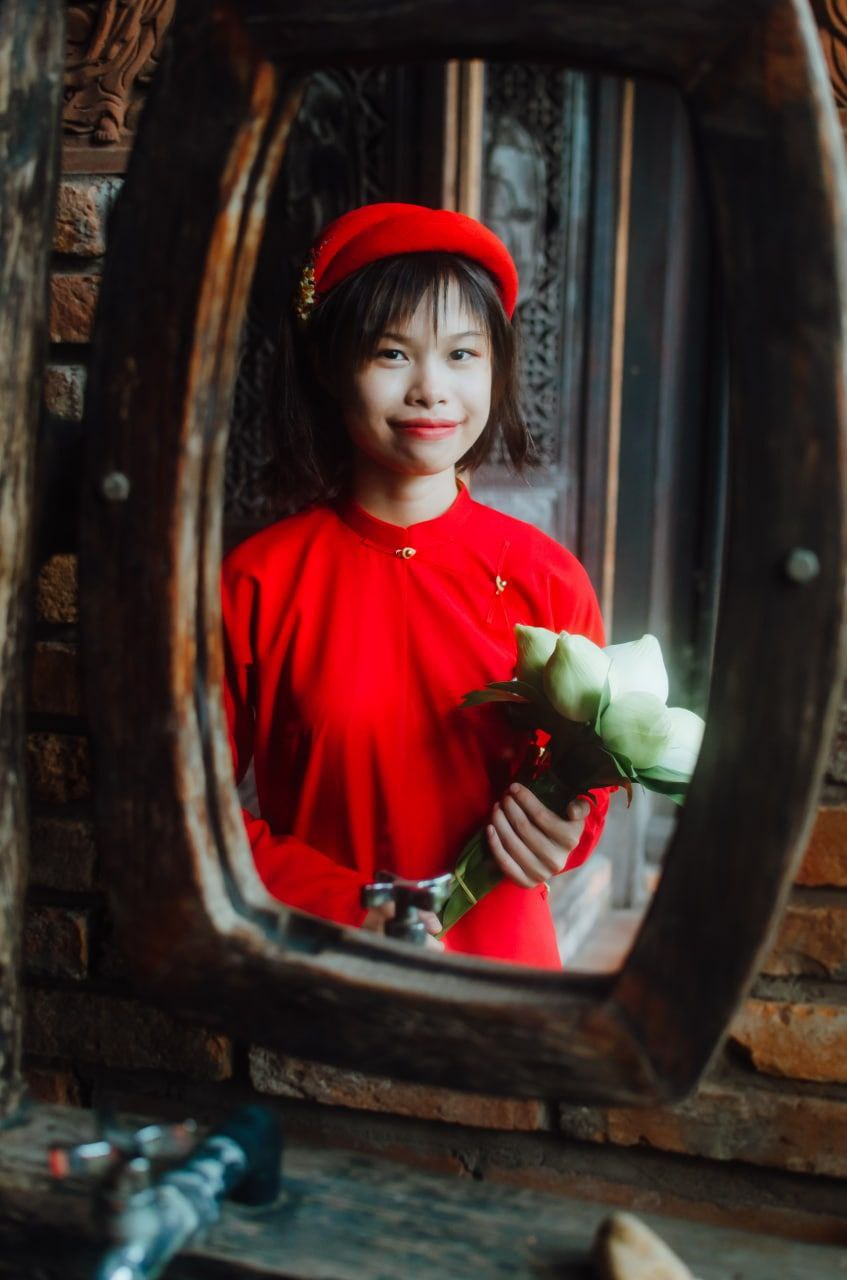
\includegraphics[width=0.6\columnwidth]{photo.jpg}\\[\baselineskip] % Your photo
\small % Smaller font size
Nguyen Viet Anh \\ % Your name
\url{nguyenvieanh2103@gmail.com} \\ % Your email address
\url{https://github.com/nguyenanh2222} \\ % Your URL
033 486 3104 \\ % Your phone number
\Sep % Some whitespace
\textbf{Address} \\
1436 Trinh Quang Nghi, Ho Chi Minh \\ % Address 1

\vfill % Whitespace under this block to push it up under the photo
\end{flushright}
}

%----------------------------------------------------------------------------------------

\begin{document}

\userinformation % Print your information in the left column

\framebreak % End of the first column

%----------------------------------------------------------------------------------------
%	HEADING
%----------------------------------------------------------------------------------------

\cvheading{Nguyen Viet Anh} % Large heading - your name

\cvsubheading{Python Developer} % Subheading - your occupation/specialization

%----------------------------------------------------------------------------------------
%	ABOUT ME
%----------------------------------------------------------------------------------------

\aboutme{About Me}
{Build, maintain, develop and manage technological system to achieve efficiency for company.Working in a professional environment and have the opportunity to develop my skills- Promote to the position of manager within 3 years.}

%----------------------------------------------------------------------------------------
%	EDUCATION
%----------------------------------------------------------------------------------------

\CVSection{Education}

%------------------------------------------------

\CVItem{2018 - 2022, Pham Ngoc Thach University}{Major in Health Care}

%------------------------------------------------

\CVItem{2021 - 2022, T3H Campus}{Learning in Python Program Language}

%------------------------------------------------

\Sep % Extra whitespace after the end of a major section

%----------------------------------------------------------------------------------------
%	EXPERIENCE
%----------------------------------------------------------------------------------------

\CVSection{Experience}

%------------------------------------------------

\CVItem{May 2022 - September, \textit{BackEnd}, EOS}{
Detailed achievements:
\begin{itemize}
	\item - Provide RESTful API for Front-end applications
        \item - Team working with code versioning tools like GitHub, GitLab
	\item - Working with Relational Database (MySQL, Postgres) as well as NoSQL (MongoDB)
 \textsc{LOS}:
	\begin{itemize}
		\item  Loan Operation System
		\item Role: Back-end
		\begin{itemize}
                \item Buil API of loan for Bank
                \item Framework: FastAPI
                \item Database: Oracle, MongoDB
                \item Design pattern three layers 
                \item eam size : 11
                \item Reposibility: Refactor API S1, map data.
			\item Windows trying to print in letter format
		\end{itemize}
		\item E-commece App
            \item Role: Back-end
            \begin{itemize}
                \item Build API of manage product
                \item Framework: FastAPI
                \item Database: Postgres
                \item Design pattern three layers 
                \item Team size : 2
                \item Reposibility: Design API
                \item \url{https://github.com/nguyenanh2222/ecommerce_oracle_database}
		\end{itemize}
	\end{itemize}
	\item Skills:
	\begin{itemize}
            \item Python: Django, FastAPI
            \item OOP: SOLID
            \item SQL: Oracle, MySQL, Postgres
            \item Java Core
	\end{itemize}
\end{itemize}
}

%------------------------------------------------

\Sep % Extra whitespace after the end of a major section


% \userinformation % Print your information in the left column
\framebreak
\framebreak
%----------------------------------------------------------------------------------------
%	CERTIFICATES
%----------------------------------------------------------------------------------------

%------------------------------------------------
\CVSection{CERTIFICATES}
\CVItem{2021, \textit{Certificate of English of IELTS 6.5}}

\CVItem{2020, \textit{Certificate of Learning Python
By: Joe Marini}, {LinkedIn Learning Certificate of Completion}}

\CVItem{2021, \textit{Learning SQL Programming
By: Joe Marini}, {LinkedIn Learning Certificate of Completion}}

\CVItem{2022, \textit{Certificate of advanced python program language By: VNU HCMC-University of Science}}

\CVItem{2022, \textit{Certificate of python program language and Django framework
By: VNU HCMC-University of Science }}

%------------------------------------------------

\Sep % Extra whitespace after the end of a major section

%----------------------------------------------------------------------------------------
%	INTERESTS
%----------------------------------------------------------------------------------------

\CVSection{Interests}

%------------------------------------------------

\CVItem{Professional}{web design, web app creation, software design, marketing}

%------------------------------------------------

\CVItem{Personal}{chess, cooking, running}

%------------------------------------------------

\Sep % Extra whitespace after the end of a major section

%----------------------------------------------------------------------------------------

\end{document}
